\documentclass[]{article}
\usepackage{lmodern}
\usepackage{amssymb,amsmath}
\usepackage{ifxetex,ifluatex}
\usepackage{fixltx2e} % provides \textsubscript
\ifnum 0\ifxetex 1\fi\ifluatex 1\fi=0 % if pdftex
  \usepackage[T1]{fontenc}
  \usepackage[utf8]{inputenc}
\else % if luatex or xelatex
  \ifxetex
    \usepackage{mathspec}
  \else
    \usepackage{fontspec}
  \fi
  \defaultfontfeatures{Ligatures=TeX,Scale=MatchLowercase}
\fi
% use upquote if available, for straight quotes in verbatim environments
\IfFileExists{upquote.sty}{\usepackage{upquote}}{}
% use microtype if available
\IfFileExists{microtype.sty}{%
\usepackage{microtype}
\UseMicrotypeSet[protrusion]{basicmath} % disable protrusion for tt fonts
}{}
\usepackage[margin=1in]{geometry}
\usepackage{hyperref}
\hypersetup{unicode=true,
            pdfborder={0 0 0},
            breaklinks=true}
\urlstyle{same}  % don't use monospace font for urls
\usepackage{graphicx,grffile}
\makeatletter
\def\maxwidth{\ifdim\Gin@nat@width>\linewidth\linewidth\else\Gin@nat@width\fi}
\def\maxheight{\ifdim\Gin@nat@height>\textheight\textheight\else\Gin@nat@height\fi}
\makeatother
% Scale images if necessary, so that they will not overflow the page
% margins by default, and it is still possible to overwrite the defaults
% using explicit options in \includegraphics[width, height, ...]{}
\setkeys{Gin}{width=\maxwidth,height=\maxheight,keepaspectratio}
\IfFileExists{parskip.sty}{%
\usepackage{parskip}
}{% else
\setlength{\parindent}{0pt}
\setlength{\parskip}{6pt plus 2pt minus 1pt}
}
\setlength{\emergencystretch}{3em}  % prevent overfull lines
\providecommand{\tightlist}{%
  \setlength{\itemsep}{0pt}\setlength{\parskip}{0pt}}
\setcounter{secnumdepth}{0}
% Redefines (sub)paragraphs to behave more like sections
\ifx\paragraph\undefined\else
\let\oldparagraph\paragraph
\renewcommand{\paragraph}[1]{\oldparagraph{#1}\mbox{}}
\fi
\ifx\subparagraph\undefined\else
\let\oldsubparagraph\subparagraph
\renewcommand{\subparagraph}[1]{\oldsubparagraph{#1}\mbox{}}
\fi

%%% Use protect on footnotes to avoid problems with footnotes in titles
\let\rmarkdownfootnote\footnote%
\def\footnote{\protect\rmarkdownfootnote}

%%% Change title format to be more compact
\usepackage{titling}

% Create subtitle command for use in maketitle
\newcommand{\subtitle}[1]{
  \posttitle{
    \begin{center}\large#1\end{center}
    }
}

\setlength{\droptitle}{-2em}

  \title{}
    \pretitle{\vspace{\droptitle}}
  \posttitle{}
    \author{}
    \preauthor{}\postauthor{}
    \date{}
    \predate{}\postdate{}
  

\begin{document}

\#\#\#\#Aplicaciones y consecuencias de las mismas

Éstos son: (3.2.1) centrados en el cliente (o \emph{front office}), que
incluyen el \emph{credit scoring}, aplicaciones en el campo de los
seguros de vida y no vida, y los chat-bots encargados de interactuar con
el cliente; (3.2.2) centrados en las operaciones (o \emph{back office}),
con casos como los modelos de gestión del riesgo y modelos de impacto de
mercado; (3.2.3) gestión de carteras y inversión en mercados
financieros; (3.2.4) casos en los que instituciones financieras y
empresas privadas aplican la IA y el aprendizaje automático en
regulación y supervisión; y (3.2.5) otras aplicaciones.

\textbf{(3.2.1) Aplicaciones front office: centradas en el cliente}

\textbf{Credit scoring}

La evaluación del crédito ha sido un método lárgamente usado por los
prestamistas a la hora de prestar o no un crédito. La capacidad de
evalúar el potencial riesgo del préstamo, otorgándole un valor, de un
determinado cliente es esencial para las compañías financieras. La
aplicación de técnicas de aprendizaje automático en este sector se está
estableciendo lárgamente entre las distintas instituciones encargadas de
prestar dinero. Tradicionalmente se han utilizado datos estructurados
como transacciones y el historial de pagos para crear modelos tales como
regresiones lineales o árboles de decisión para generar un ránking o
valoración de crédito. Sin embargo en la actualidad los prestamistas, ya
sean bancos o otras comañías, están utilizando ya otras fuentes de datos
no estructurados o semi estructurados tales como la actividad en las
redes sociales, uso del teléfono móvil o mensajes de texto. Este tipo de
datos permite a estas empresas obtener una visión más matizada de la
fiabilidad potencial que tendría un préstamo. La aplicación de modelos
de IA y ML sobre esta gran variedad de tipos de datos ha permitido a las
empresas prestamistas analizar factores cualitativos como el
comportamiento del consumo de los clientes o la valoración de la
voluntad de pagar el préstamo.

\setlength\parskip{5ex}

Una de las principales consecuencias de la capacidad de manejar
distintas fuentes de información ha sido el hecho de que actualmente es
que la segmentación de la calidad de los prestatarios se hace a mayor
escala, de una manera más rápida y más barata. En definitiva esto radica
en una \emph{decisión de crédito más rápida y acurada}
{[}@creditscoring1{]}. Otra de las consecuencias de la aplicación del
machine learning en este sector es el hecho de que puede ayudar a
garantizar un mayor acceso al crédito. Esto es así ya que los sistemas
de evaluación de crédito tradicionales necesitan una cantidad suficiente
de datos históricos sobre crédito de esa persona para poder considerarla
apta para la evaluación. Si esta información no está disponible, el
valor de la evaluación del crédito no puede ser generado y el cliente
puede ser potencialmente incapaz de obtener un crédito. Con el uso de
fuentes de datos alternativas y la aplicación de modelos de aprendizaje
automático los prestamistas son capaces de llevar a decisiones de
crédito que hubieran sido imposibles anteriormente {[}@AIboard{]}.

\setlength\parskip{5ex}

En general se pueden observar ventajas e inconvenientes de utilizar
inteligencia artificial o machine learning en el sector de la evaluación
del credito. Como ventaja se encuentra el hecho de que la IA permite
analizar una cantidad enorme de datos de una manera rápida. Esto implica
que el coste de evaluar los riesgos de los potenciales clientes se verá
reducido. Además, el hecho de introducir nuevos tipos de datos puede
permitir a las compañías el evaluar el riesgo de crédito de individuos
para los cuales no se podía evaluar utilizando los datos tradicionales
(historial de crédito). Es decir, la falta de historial de crédito o una
valoración anterior de crédito ya no serán más un impedimento a la
obtención de un crédito ya que otros indicadores de la verosimilitud del
pago están siendo utilizados por las compañías.

\setlength\parskip{5ex}

Sin embargo, el uso de complejos algoritmos de machine learning puede
conducir a una falta de transparencia con el consumidor. Cuando se
utilizan modelos de machine learning para construir una valoración o
puntuación de crédito, es generalmente más difícil el poder ofrecer una
explicación sobre esa valoración y la posterior decisión a los clientes,
auditores y supervisores. La faceta \emph{black box} que tienen
normalmente estos algoritmos lo complica. Además, ciertos autores
argumentan que la utilización de fuentes de datos alternaticvas, tales
como comportamiento online o fuentes de información financiera no
tradicionales, puede introducir \textbf{sesgo} en las decisiones de
crédito {[}@biascredit{]}. En este sentido ciertas asociaciones de
consumidores han levantado la voz en cuanto al aspecto moral. Los
modelos de machine learning pueden llevar perfiles de prestatario que
tengan en consideración la raza o el género. Por ejemplo, estos modelos
pueden puntuar a un prestatario de una minoría étnica con un mayor
riesgo por defecto sólo porque prestatarios similares han tenido
tradicionalmente unas condiciones menos favorables de crédito.

\setlength\parskip{5ex}

\textbf{Servicios de seguros}

El sector de los seguros es uno de los sectores que más confía en el
análisis de datos y la inteligencia artificial para llevar a cabo su
negocio. De hecho, el análisi estadístico representa el núcleo
fundamental de este tipo de negocio. La capacidad de evalúar el precio
de un producto asegurador es esencial para este sector para poder ser
rentable. Todas estas técnicas se basan en un análisis masivo de grandes
bases de datos que las empresas aseguradoras han venido recolectando
desde hace años para evaluar el riesgo de un potencial cliente. De esta
manera consiguen ofrecer servicios más baratos a aquellas personas con
un menor riesgo potencial o inrcementarlo para aquellas personas con más
riesgo. Un claro ejemplo que el lector es posible que haya experimentado
es el hecho de ver como incrementa la cuota de su seguro de automóvil
después de tener un accidente de tráfico.

\setlength\parskip{5ex}

Sin embargo, muchas de las aplicaciones actuales de técnicas de machine
learning incorporan el análisis de datos desestructurados para mejorar
el proceso de suscripción de los seguros, apoyando la asignación de un
precio en función de las características del potencial cliente, o para
fortalecer estrategias de márketing hacia determinados clientes
(segmentación). Ejemplos de estos nuevos tipos de datos son los datos en
tiempo real y los datos con alta granularidad. Ejemplos de estos últimos
son datos relacionados con el comportamiento de compra online o datos
telemétricos provinientes de sensores en aparatos electrónicos. En este
sentido, estas empresas empiezan a explorar cómo pueden aplicar la IA y
el machine learning sobre datos de sensores remotos, conectados a través
del \emph{Internet of Things (IoT)}, para detectar e intentar prevenir
accidentes susceptibles de ser asegurados (como accidentes de coche).

\setlength\parskip{5ex}

\textbf{Chat Bots}

Otra de las aplicaciones actuales de la inteligencia artificial en el
campo del \emph{front end} son los llamados ChatBots que se encargan de
interactuar con el cliente. Los Chat Bots son programas automáticos que
se encargan de asistir y/o ayudar a los clientes en sus transacciones
diarias o para resolver problemas. Estos programas utilizan una rama del
machine learning llamada NLP (procesamiento del lenguaje natural) para
interactuar con los clientes en lenguajes naturales, ya sea por texto o
por voz. Este tipo de programas están siendo introducidos por numerosas
compañías de servicios financieros, especialmente en sus aplicaciones
móviles o las redes sociales, con el fin de agilizar la relación con el
cliente y captar nuevas generaciones de clientes.

Actualmente los algortimos Chat Bot que se están utilizando son
relativamente sencillos y se centran en informar al cliente y resolver
cuestiones sencillas. Sin embargo, los Chat Bots se están moviendo cada
vez más hacia las recomendaciones, especialmente en las decisiones
financieras importantes. Además, este tipo de modelos permiten a las
compañías obtener información de sus clientes gracias a la interacción
con estos programas. Ejemplos de sectores que utilizan actualmente los
Chat Bots en el mundo financiero son las instituciones financieras y las
compañías de seguros. Éstas utilizan los Chat Bots para dar consejos
sobre seguros en tiempo real.

\setlength\parskip{5ex}

\textbf{(3.2.2) Aplicaciones back office: centradas en las operaciones}

\textbf{Modelos de gestión de riesgo: validación y stress-tests}

El llamado back-testing, o validación de modelos de gestión de riesgo,
es importante para el secto bancario porque ha sido utilizado
tradicionalmente para evaluar si los modelos de riesgo de los bancos
funcionan bien o no. Este tipo de modelos agrupa por ejemplo modelos de
gestión de riesgo de crédito, de liquidez, de mercado (tipo de cambio,
tipo de interés, cotización\ldots{}) o riesgo operacional. La validación
de modelos se define como el conjunto de procesos y actividades que
tienen como objetivo el verificar que los modelos, en este caso de
riesgo, están rindiendo como se esperaba, en línea con los objetivos por
los cuales se diseñaron y para evaluar su posible impacto
{[}@modeldef{]}. En este sentido, los bancos están empezando a
considerar el machine learning para poder utilizar y hacer que tenga
sentido grandes bases de datos estructurados y no estructurados y para
analizar el output de los modelos primarios. El hecho de utilizar este
gran conjunto de herramientas financieras para realizar el back-testing
o validación de modelos permite considerar cambios en el comportamiento
de los mercados y otras tendencias, con el objetivo bienintencionado de
reducir la potencial infravaloración del riesgo en distintos escenarios
financieros {[}@modeldef{]}.

\setlength\parskip{5ex}

Existen algunos ejemplos actuales de bancos que utilizan modelos de
aprendizaje automático no supervisados en sus validaciones de modelos.
Este tipo de modelos ayudan a los agentes validadores en el monitoreo
constante de los test de stress llevados a cabo internamente y de una
manera regulatoria, al ser éstos una ayuda para determinar si los
modelos de riesgo están rindiendo dentro de los límites aceptables o si
se están desviando de su objetivo principal. Además, pueden ofrecer
características o variables extra para los modelos de riesgo
operacional, tales como la vulnerabilidad de las distintas
organizaciones a los ciber ataques {[}@AIboard{]}.

\setlength\parskip{5ex}

A su vez, se está empezando a utilizar la inteligencia artificial y
técnicas de machine learning en el campo de los test de estrés
bancarios. Estas pruebas de resistencia bancaria consisten en técnicas
de simulación que tienen como objeivo determinar la capacidad de
estabilidad de una entidad bancaria. Consisten en exponer tanto las
carteras de activos como las de pasivos a diferentes situaciones para
evaluar las posibles reacciones o consecuencias. Este tipo de pruebas se
ha venido utilizando cada vez más después de la crisis financiera global
del año 2008. En este caso se utilizan modelos no supervisados de
aprendizaje automático para revisar grandes volúmenes de datos con el
objetivo de analizar cualquier sesgo en la selección de variables de
estos modelos de estrés. La consecuencia directa de la aplicación de la
IA en este tipo de pruebas es que conducen inevitablemente a mejores
modelos con mayor transparencia.

\textbf{Modelización del impacto de mercado}

El análisis de impacto de mercado consiste en evaluar el efecto que
tiene sobre los precios de mercado las acciones de compra/venta
(\emph{trading}) que hace una empresa. Para las compañías de
\emph{trading} es importante el poder evaluar el impacto que tienen
sobre los precios de mercado las operaciones que ejecutan, en especial
aquellas operaciones de gran volúmen. En este sentido es esencial para
ellas tener una estimación más precisa del impacto que tienen las
operaciones que ejecutan de manera que se pueda ajustar la periodicidad
de las mismas y minimizar los costes de ejecución de las operaciones.
Las compañías financieras están utilizando ya la IA para obtener más
información de los modelos que han utilizado históricamente, haciéndolos
más fuertes y potentes, así como para ayudar a identificar relaciones no
lineales entre las ordenes de compra y venta. Los modelos de machine
leaning que se están creando, llamados \emph{trading robots}, se
entrenan a ellos mismos para saber cómo reaccionar a los cambios en el
mercado {[}@marketimpact{]}.

\setlength\parskip{5ex}

Algunos de los ejemplos concretos de herramientas que utilizan el
machine learning para modelizar el impacto de mercado son los
siguientes. Actualmente se utiliza la IA para identificar grupos de
bonos que se comportan de manera similar. De esta manera, las compañías
pueden agrupar distintos bonos o activos financieros en grupos
utilizando técnicas de \emph{cluster} con el objetivo de poder medir y
valorar la liquidez de los bonos de manera individual. Otro de los
ejemplos de aplicación de la IA en este campo es el uso que se hace de
ella para identificar cómo la sincronización de las operaciones puede
minimizar el impacto de mercado. Estos modelos intentar evitar el hecho
de programar operaciones muy cercanas en el tiempo con el objetivo de
esquivar tener un impacto de mercado mayor que la suma de los impactos
individuales. Estos modelos se utilizan para decidir la mejor
programación de las operaciones (temporalmente hablando) y para
modificar esta programación temporal a medida que la compra venta se va
produciendo a tiempo real. Para modelizar estos cambios de utilizan
técnincas de aprendizaje automático supervisado

\textbf{(3.2.3) gestión de carteras e inversión en mercados financieros}

\textbf{Inversión y trading algorítmico}

Otro de los campos en los que se aplica actualmente la IA es en el del
\emph{trading algorítmico}. Estos sistemas de machine learning son
entrenados con información de grandes bases de datos relacionadas con
las condiciones cambiantes del mercado en cuestión y el precio para
extraer una decisión de inversión, compra o venta de una posición, y
colocarla en el mercado. Aquí entra en juego de nuevo el gran potencial
del big data y el machine learning a la hora de procesar un gran volúmen
de información de una manera muy rápida, potencialmente en tiempo real.
Estos algoritmos están constantemente analizando el mercado y posteando
acciones de compra o venta de una posición con una frecuencia muy
elevada. Es a causa de la gran velocidad en las interacciones con el
mercado generada con este tipo de sistemas que se los mercados
tradicionales se están adaptando al llamado \emph{High-Frequency Trading
(HFT)}. El \emph{trading} de alta frecuencia se soporta sobre este tipo
de algoritmos de \emph{trading} automático, que permiten alcanzar
niveles donde el ser humano no sería nunca capaz de llegar ya que no
podemos procesar tal cantidad de información de una manera tan rápida.

\setlength\parskip{5ex}

Las consecuencias de la implantación de las transacciones bursátiles de
alta fracuencia han sido tanto positivas y negativas. En primer lugar
una de las principales consecuencias positivas de la aplicación del
\emph{trading} algorítmico y la creación del llamado HFT ya ha sido
nombrada. Es el hecho de que las transacciones aumentan de velocidad. Al
ser transacciones automatizadas que se hacen de una manera rápida en
cuanto hay un cambio favorable en el mercado, también aumenta en
consecuencia el número de transacciones totales que se realizan en ese
mercado, a la par que disminuyen el número de transacciones con un mayor
volúmen. En otras palabras, transacciones de menor volúmen y más
rápidas. Otra de las consecuencias generales que se pueden apreciar es
que el hecho de introducir HFT, y la algorítmica en general, en los
mercados financieros de \emph{trading} es que se ha reducido el coste de
las transacciones. La razón es sencilla: es más barato hacer
\emph{trading} o negociación bursátil con máquinas que con humanos, por
eso el coste el coste de las transacciones se ha venido reduciendo a
medida que los mercados se han ido automatizando. En tercer lugar,
existen estudios que demuestran que la diferencia entre el precio de
compra/oferta y de venta/demanda en un mercado financiero, también
conocido como \emph{bid-ask spread}, se ha reducido a causa de la
implantación del HFT. Por consecuencia la liquidez, definida como el
valor disponible para comprar y vender dentro del rango de precios
Bid-Ask, se ha incrementado a lo largo del tiempo {[}@HFT p. 13{]}. Otra
de las consecuencias positivas del HFT se puede encontrar en términos de
estabilidad y predictibilidad de los mercados. Hay una gran evidencia
que sugiere que la eficiencia del precio, en los mercados financieros,
se ha incrementado generalmente con el crecimiento de las operaciones
bursátiles basadas en computación {[}@HFT{]}. Se ha comprovado que los
traders de HFT tienden a mover las operaciones en la dirección de los
cambios de precios permanentes (eficientes, óptimos) y en la dirección
opuesta a los precios transitorios erráticos {[}@HFTbank{]}.

\setlength\parskip{5ex}

Es totalmente cierto que, por otro lado, el hecho de incorporar las
transacciones bursátiles de alta frecuencia en los mercados financieros
ha traído, y puede provocar en el futuro, ciertas consecuencias no tan
deseables. Uno de los principales argumentos que se esgrime en numerosos
estudios en contra del HFT es que éste aumenta la volatilidad de los
mercados, aludiendo al hecho de que la volatilidad es más elevada en
mercados más rápidos. Además, al ser un sistema nuevo, es posible que
este tipo de algoritmos, que unitariamente pueden ser estables, terminen
funcionando de una manera inconsistente o muy inestable. Sin embargo,
existen toda otra serie de estudios, analizados en detalle en
{[}@AIboard{]} p.16, que ponen en evidencia una falta de eventos
empíricos que soporten esta teoría. En general los datos no confirman el
hecho de que el HFT haga que los mercados sean más volátiles. Otra de
las consecuencias negativas que podrían tener graves implicaciones,
especialmente en el futuro, es la que se puso de manifiesto el día 6 de
Mayo de 2010 en el índice E-mini S\&P 500 del mercado de futuros en
EEUU. En esta fecha se produjo lo que se llamó un \emph{Flash-Crash}, es
decir, un evento intra-día de corta duración en la que se produce un
desajuste profundo de los precios que no está generado por ningún cambio
en el valor fundamental de los activos que se están comprando/vendiendo.
En el caso del \emph{Flash-Crash} del 2010, se ejecutranon en un corto
plazo de tiempo muchos algoritmos de HFT con órdenes de venta, motivo
por el cual el precio presentó una gran volatilidad durante unos
minutos. La figura 3.5 muestra la trayectoria del precio de los futuros
en este mercado durante el crash, así como los cambios en los precios
entre transacciones consecutivas, medidos en ticks. Gracias a ella
podemos observar la gran velocidad con la que cambió el precio y la
increíble volatilidad durante este periodo.

\centering

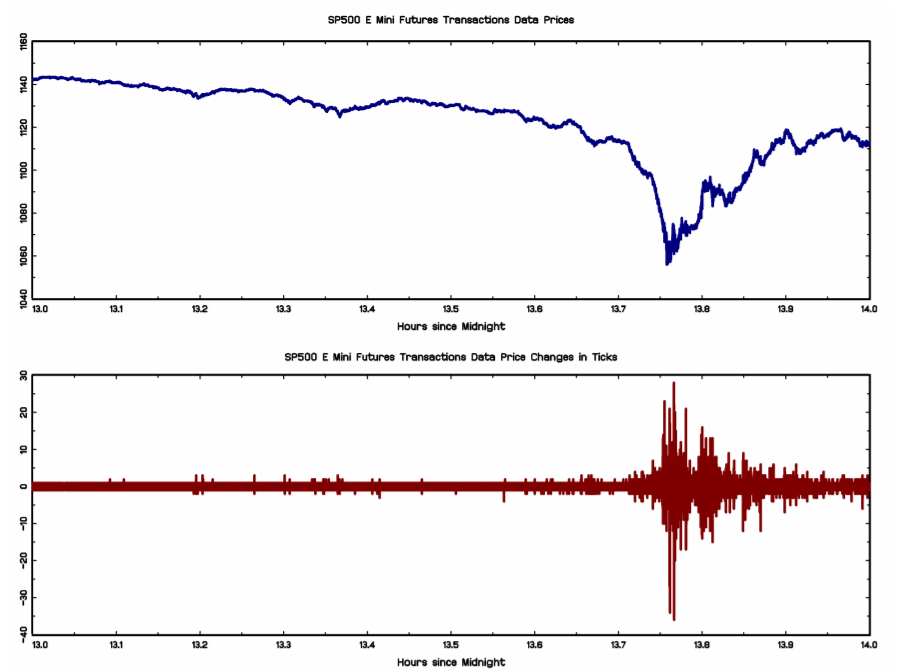
\includegraphics[width=6.77083in,height=5.20833in]{flashcrash.png}
\centering
\captionof{figure}{Nivel de precios de los futuros Emini durante el flash crash y cambios en los precios entre transacciones consecutivas. Fuente: Implications of high-frequency trading for security markets, Oliver Linton, Soheil Mahmoodzadeh 2018}

\justifying
\setlength\parskip{5ex}

Una de las posibles causas de este \emph{Flash-Crash} se encuentra
detalladamente descrita en {[}@HFT{]}. En un informe de la SEC/CFTC
(2010) se propone como punto inicial una gran orden de venta de 75000
contratos de futuros. Esto provocó que los algoritmos de trading
automático empezaran a interactuar entre ellos tratando de absorver el
gran volúmen. En general, este informe concluye que los traders de alta
frecuencia no fueron los que desencadenaron el \emph{Flash-Crash} pero
fueron sus respuestas a la presión de venta inusual generada ese día,
ejecutadas a gran velocidad, las que provocaron que la volatilidad del
mercado se viera amplificada.

\setlength\parskip{5ex}

Existen otros ejemplos de \emph{Flash-Crashes} entre los que cabe
destacar la comúnmente llamada ``Pesadilla en Wall-Street'' el 1 de
Agosto de 2012. En este caso, la compañia Knight Capital perdió
alrededor de 450 millones de dólares en unos pocos minutos a causa de un
``error de \emph{trading}'' que provocó un un desajuste transversal en
el NYSE. Otros ejemplos los podemos encontrar en los mercados de
divisas. Es el caso del llamado \emph{Sterling Flash Crash} ocurrido en
2016, donde el par GBP/USD, el tercero más líquido en el mundo,
disminuyó el valor un 9.66\% en 40 segundos {[}@HFT{]}.

\setlength\parskip{5ex}

En general, las transacciones bursátiles de alta fracuencia pueden
mejorar la calidad de los mercados, generando mayor liquidez, reduciendo
los márgenes entre precios de oferta y demanda (\emph{bid-ask spread}) y
aumentando la eficiencia. No obstante los beneficios que el HFT aporta
pueden venir con una serie de costes asociados, como ya se ha destacado.
La capacidad de estos sistemas automáticos de interactuar entre ellos de
una manera autónoma incrementa el riesgo de que se produzcan eventos
extremos que, aun siendo raros y excepcionales, se inician y desarrollan
a velocidades muy elevadas. Estas situaciones generan grandes volúmenes
de información que requieren largos periodos de tiempo para ser
analizados antes de ser entendidos.

\setlength\parskip{5ex}

\textbf{Gestión de carteras}

El uso de la inteligencia artificial y el machine learning en el sector
de la gestión de carteras es considerablemente importante. Estas
técnicas se utilizan para sacar provecho de la gran cantidad de datos
disponibles en los mercados para identificar nuevas señales en los
movimientos de los precios. Sin embargo, estas técnincas se fundamentan
en los mismos principios que las técnincas analíticas que ya se
utilizaban tradicionalmente. La idea es indentificar señales que
permitan hacer predicciones relacionadas con los precios o la
volatilidad de los \emph{stocks} para generar rentabilidades más grandes
y no correlacionadas. Especialmente se encuentra una gran implantación
en los fondos \emph{quant}, la mayoría de los cuales son fondos de
cobertura. A su vez se pueden encontrar también ejemplos de compañías
que utilizan técnicas de machine learning para recomendar a sus clientes
estrategias de inversión personalizadas y automatizadas.

\textbf{(3.2.4) Regulación y supervisión}

\textbf{Detección de fraude}

Otra de las aplicaciones actuales es en el campo de la detección de
fraudes o anomaías. Los modelos y técnicas de inteligencia artificial
ayudan a identificar conductas o comportamientos que se alejan de los
patrones regulares. Estos modelos se utilizan por ejemplo para detectar
patrones complejos y para hacer hincapié en las transacciones
sospechosas que son potencialmente más serias y peligrosas y que por lo
tanto requieren una mayor atención y cuidado. Utilizando estas técnicas
junto con distintos métodos de machine learning para analizar datos de
una manera más desagregada de transacciones, perfiles de clientes y
distintos tipos de datos desestructurados, el mundo de la inteligencia
artificial se está utilizando para descubrir relaciones no lineales
entre los diferentes atributos o características (variables), y para
detectar patrones complejos que reflejen potencialmente un blanqueo de
capitales {[}@AIboard{]}. En este sentido ayuda a agilizar el trabajo de
los agentes institucionales encargados de velar por la seguridad
financiera. Estos modelos están entrenados con una información que se
genera a tiempo real y su utilidad real está en ser capaces de detectar
y bloquear una transacción potencialmente sospechosa de fraude para su
posterior revisión. Este tipo de sistemas ha permitido ahorrar a las
autoridades y empresas un gran volúmen de masa monetaria.

\setlength\parskip{5ex}

En la actualidad existen numerosos ejemplos de empresas aplicando
tecnologías de machine learning. Casos como los de deepsense.ai o
feedzai.com son bastante habituales a día de hoy. Estas empresas se
dedican a ofrecer soluciones en relación a la detección del fraude a
otras empresas. En este modelo B2B (empresa-empresa) permite a los
clientes obtener soluciones personalizadas basadas en modelos y técnicas
de análisis de datos e inteligencia artificial para poderlos utilizar en
su día a día. También existen otros casos de empresas multinacionales
que ya han incorporado este tipo de técnicas. Es el caso de Mastercard
que lanzó en 2016 su nuevo sistema llamado ``Decision Intelligence''.
Este sistema intenta resolver la problemática de los falsos positivos de
fraude en transacciones genuinas, es decir, verdaderas, utilizando
algoritmos y técnicas de machine learning.

\textbf{Compromiso regulatorio}

Otra de las aplicaciones actuales de la inteligencia artificial y el
machine learning se puede encontrar en el campo de la regulación
financiera donde las instituciones financieras las están aplicando para
hacer más potente el compromiso regulatorio. Un ejemplo de las técnicas
que éstas utilizan son el procesamiento del lenguaje natural (NLP) para
monitorear el comportamiento y la comunicación de los \emph{traders},
con el objetivo de mantener la transparencia y la buena conducta en los
mercados. Este tipo de modelos se basan en datos tales como emails,
palabra hablada, mensajes intantáneos, documentos y otro tipo de
metadatos. A su vez, también se están utilizando los modelos de
procesamiento del lenguaje natural para interpretar, y hacer más
comprensibles, regulaciones financieras como el MiFID II. Con esto se
consigue el poder automatizar reglas de control basadas en este tipo de
regulaciones.

\textbf{(3.2.5) Otras aplicaciones}

\emph{Text mining y análisis de sentimiento}

Otra de las grandes aplicaciones de la inteligencia artificial en
general, y en especial en los sectores financieros, es la creación de
modelos de procesamiento del lenguaje natural (NLP). Las compañías
financieras y empresas FinTech ofrecen servicios basados en sistemas que
incluyen el procesamiento de todo tipo de noticias, textos en redes
sociales (social media) y arículos. La creción de regresores a partir de
información escrita potencia la capacidad predictiva de los modelos,
haciendo que sea aplicado hoy en día por numerosas empresas de servicios
de inversión. No son extraño casos como las compañías AlphaSense, Kensho
o Serimag, que ofrece servicios tales como verificación de documentos de
identificación on-line o la detección de cláusulas abusivas en las
escritura o contrato de una hipoteca
(\url{https://serimag.com/en/case-studies/}). Este tipo de modelos
consique procesar una cantidad muy elevada de información, y como se
trata de leer documentos escritos, sobrepasan enormemente la capacidad
de lectura del ser humano. Es por eso que su aplicación sigue creciendo
dentro del sector financiero y se desarrolla en nuevas herramientas o
sistemas que utilizan esta técnica.

Otra de las aplicaciones del NLP es el análisis de sentimiento. Este
conjunto de técnicas se puede considerar un subtipo de análisis dentro
del gran campo de estudio dentro del procesamiento del lenguaje natural.
Se utiliza para añadir a los modelos predictivos el punto de sentimiento
que se deriva de los textos, en general datos de redes sociales y
noticias. De esta manera se pueden construir modelos que procesen datos
a tiempo real que se pueden utilizar como proxy del estado de animo o
sentimiento de ciertos actores económicos, utilizándolos para la
predicción, por ejemplo, de la dirección de los mercados o para definir
estrategias de inversión.

\#\#\#\#Análisis económico: posibles efectos

Una vez analizadas las diferentes aplicaciones actuales de la
inteligencia artificial en el sector de las finanzas, y sus
consecuencias más directas, se procede a elaborar un análisis de las
posibles efectos o implicaciones de su implantación desde una
perspectiva económica. Concretamente se distribuye el análisis end so
partes: por un lado desde una perspectiva micro económica (o micro
financiera) y, por otro, desde una perspectiva macro económica.

\textbf{Análisis micro-económico}

En primer lugar se analizan los posibles efectos de la inteligencia
artificial en los mercados financieros. Una de los conocimientos
globales que se tiene actualmente es el hecho de que la IA y el machine
learning tienen el potencial para mejorar substancialmente la eficiencia
en el procesamiento de información. Eso deriva intevitablemente en una
reducción de las asimetrías en la información que tienen los agentes
económicos y por lo tanto puede reforzar la función de información del
sistema financiero (revisar, buscar funcion informacion sist
financiero). Los mecanismos por los cuales este refuerzo podría ocurrir
incluyen los siguientes factores. Por un lado, estos sistemas de IA
puede permitir que ciertos agentes en el mercado recojan y analicen
datos a mayor escala. Con este análisis los participantes del mercado
son potencialmente capaces de entender (mejor) la relación entre
distintos factores y la formulación de los precios de mercado. Ejemplos
de los distintos factores que se pueden relacionar con el proceso de
definición de los precios de mercado son los sentimientos o estádos de
ánimo extraídos de las redes sociales o las notícias gracias a técnicas
de \emph{sentiment analysis}. Esto podría reducir las asimetrías en la
información y de esta manera contribuir a la eficiencia y estabilidad de
los mercados (véase {[}@IOSCO{]} p.~28). Por otro lado los modelos de
machine learning e IA pueden beneficiar a los participantes en un
mercado al reducir los costes asociados a su participación. Además la IA
pude permitir a los agentes ajustar sus estrategias de inversión de una
manera casi inmediata (o en tiempo real), como respuesta a una realidad
cambiante. De esta manera se reducen en general los costes de las
transacciones en el sistema a la par que se mejora el descubrimiento de
los precios {[}@AIboard{]}. Paralelamente se observan otras
posibilidades. Si los participantes en los mercados terminan pot
utilizar técnicas similares de machine learning los riesgos
correlacionados podrían derivar en riesgos de estabilidad de los
mercados. Es decir, si el uso de \emph{traders} basados en modelos de
aprendizaje automático se empieza a ser mejor, de una manera masiva, que
el \emph{trading} clásico, esto puede provocar que muchos agentes en el
futuro decidan también utilizar este tipo de técnicas y esdevengan, en
definitiva, un sistema que puede amplificar los \emph{shocks}
financieros, tanto positivos como negativos.

En segundo lugar se analizar los posibles efectos de la IA en las
instituciones financieras. Por un lado los sistemas de machine learning
pueden mejorar los ingresos y reducir los costes para las mismas, ya que
pueden mejorar el procesamiento de distintas operaciones que este tipo
de insituciones utilizan. Al tener éstos un gran componente
computacional, el hecho de incorporar el machine learning para
automatizar y mejorar procesos de negocio rutinarios puede trasladarse
en unos costes operacionales más bajos y, en general, hacen que estas
empresas sean más rentables. Por otro lado, y como ya se ha analizado en
la presente tesis, la IA y el machine learning se pueden utilizar y se
utilizan para la gestión del riesgo. Por ejemplo, técnicas y modelos de
gestión de riesgos de cola (distribuciones de riesgos con las colas
pesadas no normales). Además también se pueden utilizar para detectar el
fraude bancario o financiero, las transacciones sospechosas y estimando
el riesgo de ciber ataques mejorando, en definitiva, el proceso de
gestión del riesgo. Sin embargo todas estas herramientas tienen un
peligro potencial ya que pueden pasar por alto nuevas fuentes de riesgo
al no estar presentes en los datos históricos utilizados para entrenar
los modelos. Otro de los posibles efectos sobre las instituciones
financieras se analiza seguidamente. El hecho de que el desarrollo en el
campo de la inteligencia artificial sea de carácter \emph{open source} y
con un uso intensivo de datos puede animar a las instituciones
financieras a colaborar con otras e incluso con otros sectores como el
comercio on-line y las economías colaborativas. En este sentido fomenta
incrementar y potencial la colaboración inter-sectorial.

No obstante todos estos efectos positivos vienen con unos riesgos
potenciales asociados. La creación de modelos de toma de decisiones
automáticas, que normalmente se convierten en cajas negras, puede hacer
dificil para las instituciones financieras el captar cómo se formulan
las decisiones, especialmente en casos de inversión y \emph{trading}
(véase {[}@black{]} para una descripción concisa de los problemas de las
\emph{black boxes} en la IA y la toma de decisiones). Esto puede derivar
en un serio problema cuando estos algoritmos causan situaciones de
\emph{Flash Crush} o cuando están relacionados con eventos extremos.
Esto sin duda significa una falta de transparencia en torno a los
sistemas de IA que puede ser problemático para las instituciones a la
hora de entender cómo y por qué han ocurrido los eventos exremos o no
deseados derivados de la aplicación de los mismos. Otro de los
potenciales riesgos de la IA es la falta de transparencia en cuanto a
las responsabilidades derivadas de las posibles pérdidas económicas en
los intermediaros que estos modelos puedan causar. Por ejemplo en el
caso de que una aplicación de IA desarrollada por un tercero provoque
grandes pérdidas. En este caso, es la institución que provoca las
gestión o movimiento la única responsable de las pérdidas? O serán las
instituciones capaces de gestionar las potenciales demandas en contra de
los desarrolladores de la aplicación? En este sentido el debate está
abiero, y habrá que seguir en el futuro las noticias relacionadas con
este tema. En este sentido, es posible que la aplicación transversal de
la IA en el sector financiero provoque cambios en la manera en la que se
regula este sector. Por último, cabe destacar las grandes dependencias
sobre terceros agentes que la aplicación de la IA en finanzas tiene. El
desarrollo de estas aplicaciones se sostiene en general gracias a un
gran número de empresas tecnológicamente avanzadas que son las
proveedoras de estos servicios. Si las grandes instituciones financieras
confían tanto en los terceros agentes, se pueden generar grandes
disrupciones en el sistema si estos terceros agentes experimentan
situaciones de alto riesgo o quiebras. Especialmente en el futuro habrá
que tener presente estos riesgos a la hora de desarrollar herramientas
de IA encargadas de misiones o tareas consideradas críticas
{[}@AIboard{]}.

En tercer lugar se analizan los potenciales efectos de la IA en los
consumidores e inversores. En general, ya se ha visto que la IA y el
machine learning tienen el potencial de reducir costes y de aumentar la
eficiencia de los servicios financieros y, por tanto, los consumidores
pueden verse beneficiados de distintas maneras. Uno de los beneficios
directos de la reducción de costes es que ésta puede verse trasladada a
los consumidores en forma de menores tasas y costes de transacción.
Además los consumidores e inversores pueden tener acceso a una mayor
variedad de servicios financieros. A su vez también pueden facilitar
unos servicios financieros mucho más customizados y personalizados ya
que la IA aplicada al big data (\emph{big data science}) permite a las
compañías analizar las características de los clientes y, así, poder
ofrecer servicios ajustados a diferentes perfiles de cliente. Sin
embargo, la utilización de estos datos de los consumidores puede llevar
a problemas de privacidad de datos y seguridad de la información (véase
{[}@privacy{]} para más información acerca de los problemas de
privacidad de dato y IA). Gracias al uso intensivo de este tipo de datos
privados los modelos de machine learning pueden llegar a ser
discriminatorios por razones de raza, sexo, religión, etc. Evitar este
tipo de modelos discriminatorios en ambientes como la evaluación del
riesgo de crédito, modelos de acceso a crédito o calculadores de cuotas
de servicios de seguros.

\textbf{Análisis macro-económico}

Macro-financial analysis Widespread adoption of AI and machine learning
could impact the financial system in a number of ways, depending on the
nature of the application. From the perspective of economic growth, the
application of AI and machine learning to financial services has
potential to enhance the efficiency of the economy and to contribute to
growth through the following mechanisms: 92 (a) Enhancing the efficiency
of financial services: more efficient risk management of individual
banks' loan portfolio and insurers' liabilities may benefit the
aggregate system. AI and machine learning could help process information
on the fundamental value of assets, thus allocating funds to investors
and projects more effectively. Moreover, if AI and machine learning
increase the speed and reduce the costs of payment and settlement
transactions, for example by executing trades at times when there are
available counterparties with corresponding demand, this may stimulate
transactions for real economic activities. (b) Facilitating
collaboration and realising new `economies of scope:' Were AI and
machine learning to facilitate collaboration between financial services
and various industries, such as e-commerce and `sharing economy'
industries, this could realise new economies of scope and foster greater
economic growth. For example, customer analysis based on transaction
data attached to payment and settlement activities (for example, ``who
buys what, when, and where?'') would encourage cooperation between
e-commerce and financial services. (c) Stimulating investments in AI and
machine learning related areas: Many firms, including non-financial
businesses, appear eager to apply AI and machine learning to their
business. The growth in investments in AI and machine learning-related
R\&D can directly contribute to economy-wide investment and thus
stimulate economic growth. From a macro-financial viewpoint, the short-
to medium-term effects of the adoption of AI and machine learning on
financial structure and markets could be more mixed. There are a number
of potential effects on the systemic importance of market participants,
the degree of concentration, and market vulnerabilities, which are
elaborated below. 5.1 Market concentration and systemic importance of
institutions AI and machine learning may affect the type and degree of
concentration in financial markets in certain circumstances. For
instance, the emergence of a relatively small number of advanced
third-party providers in AI and machine learning could increase
concentration of some functions in the financial system. Similarly,
access to big data could be a source of systemic importance, especially
if firms are able to leverage their proprietary sources of big data to
obtain substantial economies of scope. Finally, the most innovative
technologies may be mainly affordable to large companies because the
development of uses requires significant investments (for acquiring and
maintaining the infrastructure and the skilled workers). For the
possible impact of AI and machine learning on banks' systemic
importance, there are a number of key scenarios. If AI and machine
learning `unbundle' traditional banking services and entice new firms to
offer financial services, this might reduce the systemic importance of
individual large universal banks. These banks could focus on a more
narrow set of activities, rather than continuing to offer universal
services.93 However, taken as a group, universal banks' vulnerability to
systemic shocks may grow if they increasingly depend on similar
algorithms or data streams. On the other hand, if a large bank, which
already has public trust, successfully adopts AI and machine learning so
as to strengthen its market power, its systemic importance could
increase. Whether other market participants provide similar services on
competitive terms may also be affected by market entry costs and
regulation. Thus, it is difficult to assess whether AI and machine
learning would generally increase or decrease the degree of
concentration. 5.2 Potential Market Vulnerabilities Use of AI and
machine learning for trading could impact the amount and degree of
`directional' trading. Under benign assumptions, the divergent
development of trading applications by a wide range of market players
could benefit financial stability. For example, if machine
learningpowered robo-advisors give more customised advice to
individuals, their investment activities may become more tailored to
individual preferences and perhaps less correlated with other trading
strategies. By reducing the barriers to entry for retail consumers to
invest, these applications could also expand the investor base in
capital markets. Similarly, the use of AI and machine learning for new
and uncorrelated trading strategies by hedge funds could also result in
greater diversity in market movements. More efficient processing of
information could help to reduce price misalignments earlier and hence
mitigate the build-up of macro-financial price imbalances. On the other
hand, new trading algorithms based on machine learning may be less
predictable than current rule-based applications and may interact in
unexpected ways. To the extent that firms using AI or machine learning
techniques can generate higher returns or lower trading costs, it is
likely that incentives for adoption will increase. In the absence of
data on the extent of market-wide use, market movements may be ascribed
to AI and machine learning models, and interpretation of market shocks
may be hampered. Finally, high frequency trading (HFT) applications of
AI and machine learning could be new sources of vulnerabilities. If a
similar investment strategy based on AI and machine learning is widely
used in HFT, it might increase market volatility through large sales or
purchases executed almost simultaneously.94 Regarding leverage,
liquidity, and maturity transformation, the adoption of AI and machine
learning by financial market participants such as hedge funds and market
makers may also have both positive and negative impacts. AI and machine
learning could increase liquidity in financial markets through enhanced
speed and efficiency of trading activities. AI and machine learning
could be used to detect excessive risks and overly-complicated
transactions and to design more effective hedging strategies for risk
management by individual financial institutions. 95 To the extent these
tools enable the growth of new credit platforms to directly connect
lenders and borrowers (broadly called FinTech credit), 96 this could
reduce reliance on bank loans, reduce banks' leverage, and achieve a
more diversified risk-sharing structure in the overall financial system.
On the other hand, to the extent that market participants use AI and
machine learning in order to minimise capital or margins or maximise
expected returns on capital (within the constraints of regulations, and
without paying due attention to risks), the use of AI and machine
learning may increase risks. Specifically, it may allow for much tighter
liquidity buffers, higher leverage, and faster maturity transformation
than in cases where AI and machine learning had not been used for such
optimisation. 5.3 Networks and interconnectedness Applications of AI and
machine learning may enhance the interconnectedness of financial markets
and institutions in unexpected ways. Institutions' ability to make use
of big data from new sources may lead to greater dependencies on
previously unrelated macroeconomic variables and financial market
prices, including from various non-financial corporate sectors
(e-commerce, sharing economy, etc.). As institutions find algorithms
that generate uncorrelated profits or returns, there is a risk these
will be exploited on a sufficiently wide scale that correlations
actually increase. These potentially unforeseen interconnections will
only become clear as technologies are actually adopted. More generally,
greater interconnectedness in the financial system may help to share
risks and act as a shock absorber up to a point. Yet the same factors
could spread the impact of extreme shocks.97 If a critical segment of
financial institutions rely on the same data sources and algorithmic
strategies, then under certain market conditions a shock to those data
sources -- or a new strategy exploiting a widely-adopted algorithmic
strategy -- could affect that segment as if it were a single node. This
may occur even if, on the surface, the segment is made up of tens,
hundreds, or even thousands of legally independent financial
institutions. As a result, collective adoption of AI and machine
learning tools may introduce new risks. 5.4 Other implications of AI and
machine learning applications AI and machine learning applications in
insurance markets could reduce the degree of moral hazard and adverse
selection -- but could also undermine the risk pooling function of
insurance. Moral hazard and adverse selection are inherent problems in
insurance. Nonetheless, if AI and machine learning are used to
continuously adjust insurance fees in accordance with changing behaviour
of the policyholders, this may reduce moral hazard. If AI and machine
learning are utilised to offer customised insurance policies reflecting
detailed characteristics of each person, it may also decrease adverse
selection. On the other hand, these uses may pose various new
challenges. For example, the more accurate pricing of risk may lead to
higher premiums for riskier consumers (such as in health insurance for
individuals with a genetic predisposition to certain diseases) and could
even price some individuals out of the market. Even if innovative
insurance pricing models are based on large data sets and numerous
variables, algorithms can entail biases that can lead to non-desirable
discrimination and even reinforce human prejudices. This warrants a
societal discussion on the desired extent of risk sharing, how the
algorithms are conceived, and which information is admissible.98
Meanwhile, AI and machine learning can continue to be a useful tool both
for financial institutions (RegTech) and supervisors (SupTech). Many of
the uses described in section 3.4 could result in improvements in risk
management, compliance, and systemic risk monitoring, while potentially
reducing regulatory burdens. Yet, if a similar type of AI and machine
learning is used without appropriately `training' it or introducing
feedback, reliance on such systems may introduce new risks. For example,
if AI and machine learning models are used in stress testing without
sufficiently long and diverse time series or sufficient feedback from
actual stress events, there is a risk that users may not spot
institution-specific and systemic risks in time. These risks may be
pronounced especially if AI and machine learning are used without a full
understanding of the underlying methods and limitations. Furthermore, as
the current regulatory framework is not designed with the use of such
tools in mind, some regulatory practices may need to be revised for the
benefits of AI and machine learning techniques to be fully harnessed.
For example, in MiFID II, where an obligation is placed on the firm to
submit a report when a reportable event occurs, regulatory compliance is
expected of the firm at all times. If AI and machine learning tools are
used to deem if a particular activity is reportable or not, mistakes
would still result in regulatory action, even if the tools can identify
what information the regulators truly needs in order to reduce the risk
of market disruption. In this regard, combining AI and machine learning
with human judgment and other available analytical tools and methods may
be more effective, particularly to facilitate causal analysis. 99 More
generally, the greater adoption of AI, machine learning, and other
technological advances in finance may benefit also from more of a
`systems' perspective in financial regulation to contribute to financial
stability in an increasingly complex system. 100 If optimisation
solutions are adopted primarily by the private sector but not the public
sector, there may be a risk that some individuals or firms may use them
more successfully to `game' regulatory rules or conduct regulatory
arbitrage.

REVISAR Faster and cheaper financial decisions

chatbots--\textgreater{} give less human relation in financial sector

the use of personal data raises other policy issues, including those
related to data privacy and data protections

While the use of machine learning has the potential to produce more
accurate pricing and risk assessment for insurance companies, there may
be consumer protection concerns that stem from potential data errors or
the exclusion of some groups (see section 5).

Mayor seguridad financiera, mayor control


\end{document}
